\documentclass[../main]{subfiles}

\begin{document}
\chapter{Miscellaneous}
\section{C++}
\subsection{Structure Member Alignment and Padding}
\subsubsection{Data alignment in memory}
    Every data type in C will have alignment requirements (in fact it is mandated by processor architecture, not by language).
A processor will have processing word length as that of data bus size. On a 32-bit machine, the processing word size will be 4 bytes.\newline

    Historically, memory is byte-addressable and arranged sequentially. If the memory is arranged as a single bank of one-byte width,
the processor needs to issue 4 memory read cycles to fetch an integer. It is more economical to read all 4 bytes of an integer in one memory cycle.
To take such advantage, the memory will be arranged as a group of 4 banks as shown below.
\begin{center}
    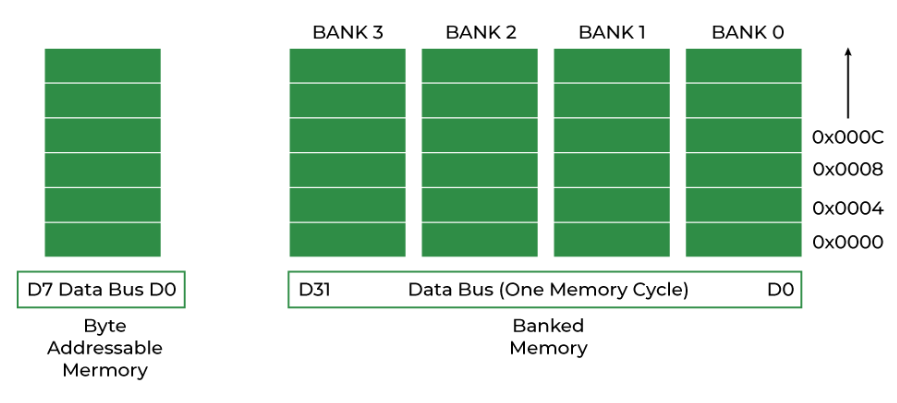
\includegraphics[scale=0.7]{Pictures/banks.png}
\end{center}

    The memory addressing still be sequential. If bank 0 occupies an address X, bank 1, bank 2 and bank 3 will be at $(X + 1)$, $(X + 2)$, and $(X + 3)$ addresses.
If an integer of 4 bytes is allocated on $X$ address (X is a multiple of 4), the processor needs only one memory cycle to read the entire integer.
Whereas, if the integer is allocated at an address other than a multiple of 4, it spans across two rows of the banks as shown in the below figure.
Such an integer requires two memory read cycles to fetch the data.
\begin{center}
    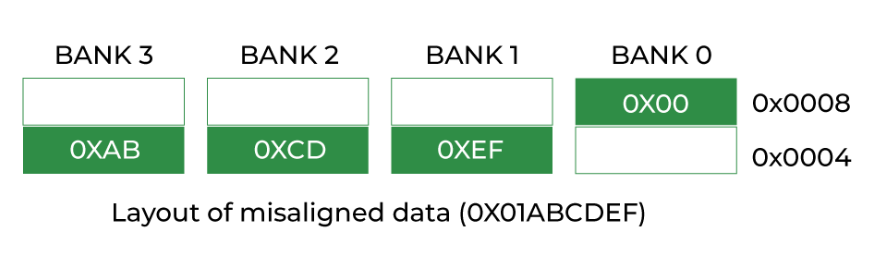
\includegraphics[scale=0.7]{Pictures/misaligned.png}
\end{center}

    A variable’s data alignment deals with the way the data is stored in these banks. For example, the natural alignment of \texttt{int} on a 32-bit machine is 4 bytes.
When a data type is naturally aligned, the CPU fetches it in minimum read cycles. Similarly, the natural alignment of a short int is 2 bytes. It means a short \texttt{int} can be stored
in bank 0 – bank 1 pair or bank 2 – bank 3 pair. A \texttt{double} requires 8 bytes and occupies two rows in the memory banks.
Any misalignment of double will force more than two read cycles to fetch double data.\newline

Note that a \texttt{double} variable will be allocated on an 8-byte boundary on a 32-bit machine and requires two memory read cycles.
On a 64-bit machine, based on a number of banks, a \texttt{double} variable will be allocated on the 8-byte boundary and requires only one memory read cycle.

\subsubsection{Structure padding}
    Structure padding is the addition of some empty bytes of memory in the structure to naturally align the data members in the memory.
It is done to minimize the CPU read cycles to retrieve different data members in the structure. Let's start with calculating the size of a few types
\begin{Code}
    #include <iostream>
    
    int main()
    {
        /* Prints "1" */
        std::cout << sizeof(char) << std::endl;
        
        /* Prints "2" */
        std::cout << sizeof(short int) << std::endl;
        
        /* Prints "4" */
        std::cout << sizeof(int) << std::endl;
        
        /* Prints "8" */
        std::cout << sizeof(double) << std::endl;
    
        return 0;
    }
\end{Code}

    Okay, we know how wide these types are so now, let's define a few structures
\begin{Code}
    #include <iostream>
    
    struct Struct1
    { 
        char c; 
        short int s; 
    }; 
      
    struct Struct2
    { 
        short int s; 
        char c; 
        int i; 
    }; 
      
    struct Struct3
    { 
        char c; 
        double d; 
        int s; 
    }; 
      
    struct Struct4
    { 
        double d; 
        int s; 
        char c; 
    };
    
    int main()
    {
        Struct1 struct1 {};
        Struct2 struct2 {};
        Struct3 struct3 {};
        Struct4 struct4 {};
        
        std::cout << sizeof(struct1) << std::endl;
        std::cout << sizeof(struct2) << std::endl;
        std::cout << sizeof(struct3) << std::endl;
        std::cout << sizeof(struct4) << std::endl;
        
        return 0;
    }
\end{Code}
\noindent
We may expect that
\begin{itemize}
    \item \texttt{sizeof(struct1)} = 1 + 2 = 3,
    \item \texttt{sizeof(struct2)} = 2 + 1 + 4 = 7,
    \item \texttt{sizeof(struct3)} = 1 + 8 + 4 = 13,
    \item \texttt{sizeof(struct4)} = 8 + 4 + 1 = 13,
\end{itemize}
\noindent
but the reality is
\begin{itemize}
    \item \texttt{sizeof(struct1)} = 4, 
    \item \texttt{sizeof(struct2)} = 8,
    \item \texttt{sizeof(struct3)} = 24,
    \item \texttt{sizeof(struct4)} = 16.
\end{itemize}

    The results are different than expected \textbf{because of the alignment requirements of various data types - every member of the structure should be naturally aligned so
the members of the structure are allocated sequentially in increasing order.} Let us analyze each struct
\begin{itemize}
    \item \textbf{\texttt{Struct1}} - the first element is \texttt{char} which is 1 byte aligned, followed by \texttt{short int} which is 2 bytes aligned.
    If the short int element is immediately allocated after the char element, it will start at an odd address boundary. The compiler will insert a \textbf{\textit{padding byte}}
    after the \texttt{char} to ensure \texttt{short int} will have an address multiple of 2 (i.e. 2 byte aligned). The total size of \texttt{Struct1} will be
    \begin{center}
        \texttt{sizeof(char)} + \textbf{\textit{padding byte}} + \texttt{sizeof(short int)} = 4.
    \end{center}
    \item \textbf{\texttt{Struct2}} - the first element is \texttt{short} 2 byte aligned. Since \texttt{char} can be on any byte boundary, no padding is required between these types.
    But the next one is \texttt{int} which is 4 byte aligned, thus it cannot start at an odd byte boundary, so one padding byte is needed. Therefore,
    \begin{center}
        \texttt{sizeof(short int)} + \texttt{char} + \textbf{\textit{padding byte}} + \texttt{int} = 8.
    \end{center}
    \item \textbf{\texttt{Struct3}} - Observe that after adding padding byte after \texttt{char} we are not on the byte that is the multiplication of \texttt{sizeof(double)} = 8, so we need
    to add seven padding bytes to it, thus
    \begin{center}
        \texttt{char} + 7 * \textbf{\textit{padding byte}} + \texttt{double} + \texttt{int} = 20.
    \end{center} However, the size of the structure is 24. What happened? This is because structure-type variables also have natural alignment, for instance
    \begin{Code}
        Struct3 structs[3];
    \end{Code}
    Assume that the base address of \texttt{structs[0]} is 0. The whole \texttt{Struct3} has a size equal to 20, so the second element \texttt{structs[1]} starts with
    20 address, and therefore, the \texttt{double} member must start from 28 which is not the dividend of 8 (size of \texttt{double}). To avoid that,
    \textbf{the compiler introduces alignment requirements to every structure}, so in this case it needs to add \textbf{four padding bytes} to make
    the structure size multiple of its alignment. Eventually
    \begin{center}
        \texttt{char} + 7 * \textbf{\textit{padding byte}}  + \texttt{double} + \texttt{int} + 4 * \textbf{\textit{padding byte}}  = 24.
    \end{center}
    \item \textbf{\texttt{Struct4}} - we have
    \begin{center}
        \texttt{sizeof(double)} + \texttt{sizeof(int)} + \texttt{sizeof(char)} = 13
    \end{center}
    but because of \texttt{double} size, we need to add 3 padding bytes, then we have 16.
\end{itemize}

    Structure padding is not avoidable, but can be easily optimized - it is enough to \textbf{declare the structure members in their increasing or decreasing order of size}.
It is visible in the examples of \texttt{Struct3} and \texttt{Struct4}.

\subsection{Value categories}
\subsubsection{C++11}
    Since C++11 we have the following \textbf{core categories of values}
\begin{itemize}
    \item \textbf{\textit{lvalue}}, for instance
    \begin{itemize}
        \item an expression that is just the name of a variable, function, or member.
        \item an expression that is just a string literal.
        \item the result of the built-in unary \texttt{*} operator (i.e., dereferencing operator).
        \item the result of a function returned by \textbf{lvalue} reference.
    \end{itemize}
    \item \textbf{\textit{prvalue}} - \textit{pure rvalue}, for instance
    \begin{itemize}
        \item expressions that consist of a literal that \textbf{is not a string literal} or a user-defined literal, where the return type
        of the associated literal operator defines the category.
        \item the result of the built-in unary \texttt{\&} operator (i.e., taking an address of an expression).
        \item the result of built-in arithmetic operators.
        \item the result of a function returned by value.
        \item a lambda expression.
    \end{itemize}
    \item \textbf{\textit{xvalue}} - \textit{expiring value}, for instance
    \begin{itemize}
        \item the result of a function returned by \textbf{rvalue} reference, especially returned by \texttt{std::move()},
        \item a cast to an \textbf{rvalue} reference to an object type,
    \end{itemize}
\end{itemize}

    From the above, we can get a brief conclusion
\begin{itemize}
    \item All names used as expressions are \textbf{lvalues}.
    \item All string literals used as expressions are \textbf{lvalues}.
    \item All other literals (\texttt{4.2}, \texttt{true}, \texttt{nullptr}, etc) are \textbf{prvalues}.
    \item All temporaries, especially objects returned by value, are \textbf{prvalues}.
    \item The result of \texttt{std::move()} is an \textbf{xvalue}.
\end{itemize}

    The composite values are
\begin{itemize}
    \item \textbf{\textit{glvalue}} (\textit{generalized value} which is the union of \textbf{lvalue} and \textbf{xvalue}),
    \item \textbf{\textit{rvalue}} (the union of \textbf{xvalue} and \textbf{prvalue}).
\end{itemize}

    All of these types create the following structure
\begin{center}
    \begin{tikzcd}
                        &                                        & \textbf{Expression} \arrow[ld] \arrow[rd] &                                       &                 \\
                        & \textbf{glvalue} \arrow[ld] \arrow[rd] &                                           & \textbf{rvalue} \arrow[ld] \arrow[rd] &                 \\
        \textbf{lvalue} &                                        & \textbf{xvalue}                           &                                       & \textbf{prvalue}
    \end{tikzcd}
\end{center}

    It needs to be emphasized, that \textbf{glvalues}, \textbf{prvalues} and \textbf{xvalues} are \textbf{terms for expressions and not for values}, so these
names are a bit misleading. For instance, a variable itself isn't an \textbf{lvalue}, only the expression denoting the variable is \textbf{lvalue}
\begin{Code}
    int i = 3;  // i is a variable, not an lvalue
    int j = i;  // i is lvalue in this expression
\end{Code}

\subsubsection{C++17}
    C++17 didn't change these value categories, so it stays as it was, but clarifies their semantic meaning
\begin{center}
    \begin{tikzcd}
                    &                                        & \textbf{Expression} \arrow[ld] \arrow[rd]                 &                                       & \\
                    & \textbf{glvalue} \arrow[ld] \arrow[rd] &                                                           & \textbf{rvalue} \arrow[ld] \arrow[rd] & \\
        \textbf{lvalue} &                                    & \textbf{xvalue} &               & \textbf{prvalue} \arrow[ll, "materialization"', dashed] 
    \end{tikzcd}
\end{center}

    To explain value categories now is that in general, we have two kinds of expressions
\begin{itemize}
    \item \textbf{glvalues} - expressions for \textbf{locations of object or functions},
    \item \textbf{prvalues} - expressions for \textbf{initializations}.
\end{itemize}
\noindent
An \textbf{xvalue} is then considered a special location, representing an object whose resources can be reused, usually because it is near the end of its lifetime.
The new thing in C++17 is the term \textbf{materialization}, for the moment a \textbf{prvalue} becomes a temporary object.
Thus, a temporary materialization conversion is a \textbf{prvalue} $\rightarrow$ \textbf{xvalue} conversion.\newline

\section{General}
\subsection{Bit and Byte}
\noindent
\textbf{Bit} is the smallest unit of storage. Its value is either 0 or 1.\newline
\textbf{Byte} is a collection of 8 bits.

\subsection{Big Endian and Little Endian}
    Endianness refers to the order in which bytes are stored in memory for multi-byte data types
(such as integers and floating-point numbers). The two main types of endianness are \textbf{big endian} and \textbf{little endian}. For example
consider a 4-byte integer
\begin{equation}
    \text{num} = 0x12345678
\end{equation}
The hexadecimal number \texttt{0x12345678} consists of four bytes
\begin{center}
\texttt{0x12}, \texttt{0x34}, \texttt{0x56}, \texttt{0x78}
\end{center}
The way these bytes are stored in memory depends on the system's endianness.

\subsubsection{Big Endian}
    In a big-endian system, the \textbf{most significant byte (MBS)} is stored at the lowest memory address (first).
The bytes are stored in the same order as they appear in the number
\begin{center}
    \begin{tabular}{|c|c|c|c|c|}
    \hline
    Address & Byte \#1 & Byte \#2 & Byte \#3 & Byte \#4 \\
    \hline
    1000 & 0x12 & 0x34 & 0x56 & 0x78 \\
    \hline
    \end{tabular}
\end{center}
This is the convention used by some architectures like Motorola 68k and SPARC.

\subsubsection{Little Endian}
In a little-endian system, the \textbf{least significant byte (LSB)} is stored at the lowest memory address (first).
The bytes are stored in reverse order regarding the previous case
\begin{center}
    \begin{tabular}{|c|c|c|c|c|}
    \hline
    Address & Byte \#1 & Byte \#2 & Byte \#3 & Byte \#4 \\
    \hline
    1000 & 0x78 & 0x56 & 0x34 & 0x12 \\
    \hline
    \end{tabular}
\end{center}
This is the convention used by x86 and ARM processors in little-endian mode.\newline

\subsection{Compiler and Linker}
\subsubsection{Compiler}
    A \textbf{compiler} is a program that translates high-level source code
(written in languages like C, C++, Java, etc.) into a lower-level language that
a computer can understand, typically machine code or assembly language.
Its major responsibilities are
\begin{enumerate}
    \item \textbf{Lexical Analysis:} Breaks the code into tokens (like keywords, variables, and symbols).
    \item \textbf{Syntax Analysis:} Checks if the structure of the code follows the rules of the programming language.
    \item \textbf{Semantic Analysis:} Ensures the code makes logical sense (e.g., type-checking and variable declarations).
    \item \textbf{Intermediate Code Generation:} Creates an abstract, simplified version of the code.
    \item \textbf{Optimization:} Improves the code for better performance (e.g., reducing unnecessary instructions or eliminating redundant computations).
    \item \textbf{Code Generation:} Converts the optimized intermediate code into machine code or assembly language.
\end{enumerate}

    The output of the compiler is usually an \textbf{object file}
(e.g., \texttt{.o} or \texttt{.obj}), which contains machine code but
is not yet executable. Some compilers also generate debugging information,
which can assist in troubleshooting during the later stages of development.

\subsubsection{Linker}
    A \textbf{linker} is a program that combines the object files
produced by the compiler into a single executable file that can run on a computer. Its responsibilities are

\begin{enumerate}
    \item \textbf{Combining Object Files:} Links together multiple object files (e.g., from different source files or libraries) into a single program.
    \item \textbf{Resolving Symbols:} Matches function calls and variable references to their definitions. For example, if we call a function defined in another file, the linker ensures the correct function is used.
    \item \textbf{Library Handling:} Links in additional libraries (such as the standard library or third-party libraries) that our program depends on.
    \item \textbf{Address Assignment:} Determines the memory locations for functions, variables, and other components of the program.
    \item \textbf{Final Output:} Produces an executable file (e.g., \texttt{.exe} on Windows or an ELF file on Linux) that the operating system can load and execute.
\end{enumerate}

    The linker also ensures that all external references (e.g., function calls,
global variables) are resolved and all necessary components are included. If any required symbols or files are missing, the linker will generate errors, preventing the creation of the executable.

\subsection{Computational and memory complexity}
Computational and memory complexity are concepts used in computer science and algorithm analysis to evaluate the efficiency of algorithms in terms of their performance and resource requirements.

\subsubsection{Computational Complexity}
Computational complexity measures \textbf{how many computational operations an algorithm needs to perform} to solve a task for input data of a given size.
It describes how the runtime of the algorithm increases with the size of the input data. We have three main types of Computational Complexity:
\begin{itemize}
    \item \textbf{Worst case} – analyzes the runtime of the algorithm in the worst possible scenario.
    \item \textbf{Average case} – analyzes the runtime of the algorithm in an "average" scenario.
    \item \textbf{Best case} – analyzes the runtime of the algorithm in the most optimistic scenario.
\end{itemize}

    Asymptotic notation (e.g., Big-O notation) is used to describe how the runtime of the algorithm changes for large input sizes, for example
\begin{itemize}
    \item \(\mathcal{O}(1)\) – Constant complexity: the runtime of the algorithm does not depend on the size of the input.
    \item \(\mathcal{O}(\log n)\) – Logarithmic complexity: the algorithm becomes faster for large inputs (e.g., binary search).
    \item \(\mathcal{O}(n)\) – Linear complexity: the runtime grows proportionally to the number of input elements.
    \item \(\mathcal{O}(n^2)\) – Quadratic complexity: the algorithm performs operations proportional to the square of the input size (e.g., bubble sort).
    \item \(\mathcal{O}(2^n)\) – Exponential complexity: the algorithm becomes very slow even for small inputs (e.g., brute-force solution to the traveling salesman problem).
\end{itemize}

\subsubsection{Memory Complexity}
Memory complexity measures \textbf{how much memory an algorithm needs} to process input data of a given size. It includes memory used by:
\begin{enumerate}
    \item Input data,
    \item Auxiliary variables,
    \item Data structures used in the algorithm (e.g., stacks, queues),
    \item Recursive function calls.
\end{enumerate}
There are two main categories
\begin{itemize}
    \item \textbf{Fixed memory:} Occupied by variables whose size does not depend on the input size.
    \item \textbf{Dynamic memory:} Occupied by data structures that grow with the input size.
\end{itemize}

Some examples should clarify the explanation above
\begin{itemize}
    \item \(\mathcal{O}(1)\): The algorithm requires a constant amount of memory, regardless of the input size.
    \begin{itemize}
        \item Example: Calculating the average of an array (summing elements).
    \end{itemize}
    \item \(\mathcal{O}(n)\): The algorithm requires memory proportional to the input size.
    \begin{itemize}
        \item Example: Copying an array.
    \end{itemize}
    \item \(\mathcal{O}(n^2)\): The algorithm requires memory proportional to the square of the input size.
    \begin{itemize}
        \item Example: A two-dimensional array for matrix computations.
    \end{itemize}
\end{itemize}

\pagebreak 

\subsubsection{Comparison of Computational and Memory Complexity}
\begin{table}[h!]
    \centering
    \begin{tabular}{|c|c|c|}
        \hline
        \textbf{Category} & \textbf{Computational Complexity} & \textbf{Memory Complexity} \\
        \hline
        What it measures? & Number of computational operations & Amount of memory required \\
        \hline
        Unit of measurement & Operations & Memory units (e.g., bytes) \\
        \hline
        Notation & \(\mathcal{O}(n), \mathcal{O}(\log n), \mathcal{O}(n^2), \ldots\) & \(\mathcal{O}(1), \mathcal{O}(n), \mathcal{O}(n^2), \ldots\) \\
        \hline
    \end{tabular}
\end{table}

\subsection{Computational and Memory Complexity for STL containers}

\fontsize{10.3}{13}\selectfont
\begin{longtable}{|l|l|l|l|}
\hline
\textbf{Container} & \textbf{Operation} & \textbf{Time} & \textbf{Space} \\
\hline
\endfirsthead
\hline
\textbf{Container} & \textbf{Operation} & \textbf{Time} & \textbf{Space} \\
\hline
\endhead
\hline
\endfoot
\hline

\textbf{std::vector} & Insert (end) & $O(1)$ amortized & $O(n)$ \\
 & Insert (middle) & $O(n)$ & $O(n)$ \\
 & Delete (end) & $O(1)$ & $O(n)$ \\
 & Delete (middle) & $O(n)$ & $O(n)$ \\
 & Search (by index) & $O(1)$ & $O(1)$ \\
 & Search (value) & $O(n)$ & $O(n)$ \\
\hline

\textbf{std::deque} & Insert (end) & $O(1)$ amortized & $O(n)$ \\
 & Insert (beginning) & $O(1)$ amortized & $O(n)$ \\
 & Insert (middle) & $O(n)$ & $O(n)$ \\
 & Delete (end) & $O(1)$ & $O(n)$ \\
 & Delete (beginning) & $O(1)$ & $O(n)$ \\
 & Delete (middle) & $O(n)$ & $O(n)$ \\
 & Search (value) & $O(n)$ & $O(n)$ \\
\hline

\textbf{std::list} & Insert (anywhere) & $O(1)$ with iterator & $O(n)$ \\
(Doubly Linked List) & Delete (anywhere) & $O(1)$ with iterator & $O(n)$ \\
 & Search (value) & $O(n)$ & $O(n)$ \\
\hline

\textbf{std::forward\_list}& Insert (anywhere) & $O(1)$ with iterator & $O(n)$ \\
(Singly Linked List) & Delete (anywhere) & $O(1)$ with iterator & $O(n)$ \\
 & Search (value) & $O(n)$ & $O(n)$ \\
\hline

\textbf{std::set} & Insert (unique) & $O(\log n)$ & $O(n)$ \\
(Balanced Binary Search Tree) & Delete (by value) & $O(\log n)$ & $O(n)$ \\
 & Search (value) & $O(\log n)$ & $O(n)$ \\
\hline

\textbf{std::multiset} & Insert (duplicates allowed) & $O(\log n)$ & $O(n)$ \\
(Balanced Binary Search Tree) & Delete (all instances) & $O(\log n)$ & $O(n)$ \\
 & Search (value) & $O(\log n)$ & $O(n)$ \\
\hline

\textbf{std::unordered\_set} & Insert (unique) & $O(1)$ average, $O(n)$ worst & $O(n)$ \\
(Hash table) & Delete (by value) & $O(1)$ average, $O(n)$ worst & $O(n)$ \\
 & Search (value) & $O(1)$ average, $O(n)$ worst & $O(n)$ \\
\hline

\textbf{std::map} & Insert (key-value) & $O(\log n)$ & $O(n)$ \\
(Balanced Binary Search Tree) & Delete (by key) & $O(\log n)$ & $O(n)$ \\
 & Search (by key) & $O(\log n)$ & $O(n)$ \\
\hline

\textbf{std::multimap} & Insert (duplicates allowed) & $O(\log n)$ & $O(n)$ \\
(Balanced Binary Search Tree) & Delete (all instances) & $O(\log n)$ & $O(n)$ \\
 & Search (by key) & $O(\log n)$ & $O(n)$ \\
\hline

\textbf{std::unordered\_map} & Insert (key-value) & $O(1)$ average, $O(n)$ worst & $O(n)$ \\
(Hash Table) & Delete (by key) & $O(1)$ average, $O(n)$ worst & $O(n)$ \\
 & Search (by key) & $O(1)$ average, $O(n)$ worst & $O(n)$ \\
\hline

\textbf{std::stack} & Push & $O(1)$ & $O(n)$ \\
(Uses std::deque) & Pop & $O(1)$ & $O(n)$ \\
 & Top & $O(1)$ & $O(1)$ \\
\hline

\textbf{std::queue} & Enqueue (push) & $O(1)$ & $O(n)$ \\
(Uses std::deque) & Dequeue (pop) & $O(1)$ & $O(n)$ \\
 & Front & $O(1)$ & $O(1)$ \\
\hline

\textbf{std::priority\_queue} & Insert (push) & $O(\log n)$ & $O(n)$ \\
(Heap based) & Delete (pop top) & $O(\log n)$ & $O(n)$ \\
 & Top & $O(1)$ & $O(1)$ \\
\hline
\end{longtable}
\normalsize

\subsection{CPU cache and preferching}
    A \textbf{CPU cache} is a hardware cache used by the central processing unit (CPU) of a computer to reduce the average cost (time or energy)
to access data from the main memory. A cache is a smaller, faster memory, located closer to a processor core, which stores copies of the data from frequently used main memory locations.
Most CPUs have a hierarchy of multiple cache levels (L1, L2, often L3, and rarely even L4), with different instruction-specific and data-specific caches at level 1. The cache memory is typically implemented with a static random-access memory (SRAM), in modern CPUs by far the largest part of them by chip area, but SRAM is not always used for all levels
(of I- or D-cache), or even any level, sometimes some latter or all levels are implemented with eDRAM.\newline

    When trying to read from or write to a location in the main memory, the processor checks whether the data from that location is already in the cache.
If so, the processor will read from or write to the cache instead of the much slower main memory.\newline

    \textbf{Cache prefetching} is a technique used by computer processors to boost execution performance by fetching instructions or data from their original storage in slower
memory to a faster local memory before it is actually needed (hence the term 'prefetch'). Most modern computer processors have fast and local cache memory in which prefetched
data is held until it is required. The source for the prefetch operation is usually the main memory. Because of their design, accessing cache memories is typically
much faster than accessing main memory, so prefetching data and then accessing it from caches is usually many orders of magnitude faster than accessing it directly from main memory.
Prefetching can be done with non-blocking cache control instructions.\newline

    Cache prefetching can be accomplished either by hardware or by software.
\begin{enumerate}
    \item \textbf{Hardware-based prefetching} is typically accomplished by having a dedicated hardware mechanism in the processor that watches the stream of
    instructions or data being requested by the executing program, recognizes the next few elements that the program might need based on this stream and
    prefetches into the processor's cache.
    \item \textbf{Software-based prefetching} is typically accomplished by having the compiler analyze the code and insert additional prefetch instructions
    in the program during compilation itself.
\end{enumerate}
\end{document}